%!TEX root = ../dissertation.tex

\chapter{Methodology}
\label{methodology}

EXPLAIN NOTATION ROT MAT COORDINATE SYSTEM USED WHY

\section{Approach}

Figure \ref{cha3:methodology:approach} summarizes the approach that this work will take to deal with determining the orientation of the camera. The coming paragraph gives a brief overview on each of the parts of the procedure, that will be further detailed afterwards.

\begin{enumerate}
	\item \textbf{Collect images}\\
	 Using an uEye LE USB3 camera \footnote{See appendix \ref{appendix:cha2:camera} for camera specifications.}, two grayscale images are collected before and after a certain rotation.
	 
	 \item \textbf{Collect ground truth}\\
	 Using the same camera in the same positions, the two images are taken but positioning a chessboard \footnote{See appendix \ref{appendix:cha2:chessboard} for chessboard specifications.} on the scenery, which is used to determine the ground truth through its regular pattern. The ground truth will then be utilized to evaluate the estimation algorithms performance and also the \acrshort{imu}'s performance over the camera.\\
	 
	 On Figure \ref{cha3:methodology:imagesex}, an example of the two image pairs that are collected can be observed.
	 
\begin{figure}[ht]
	 \centering
	 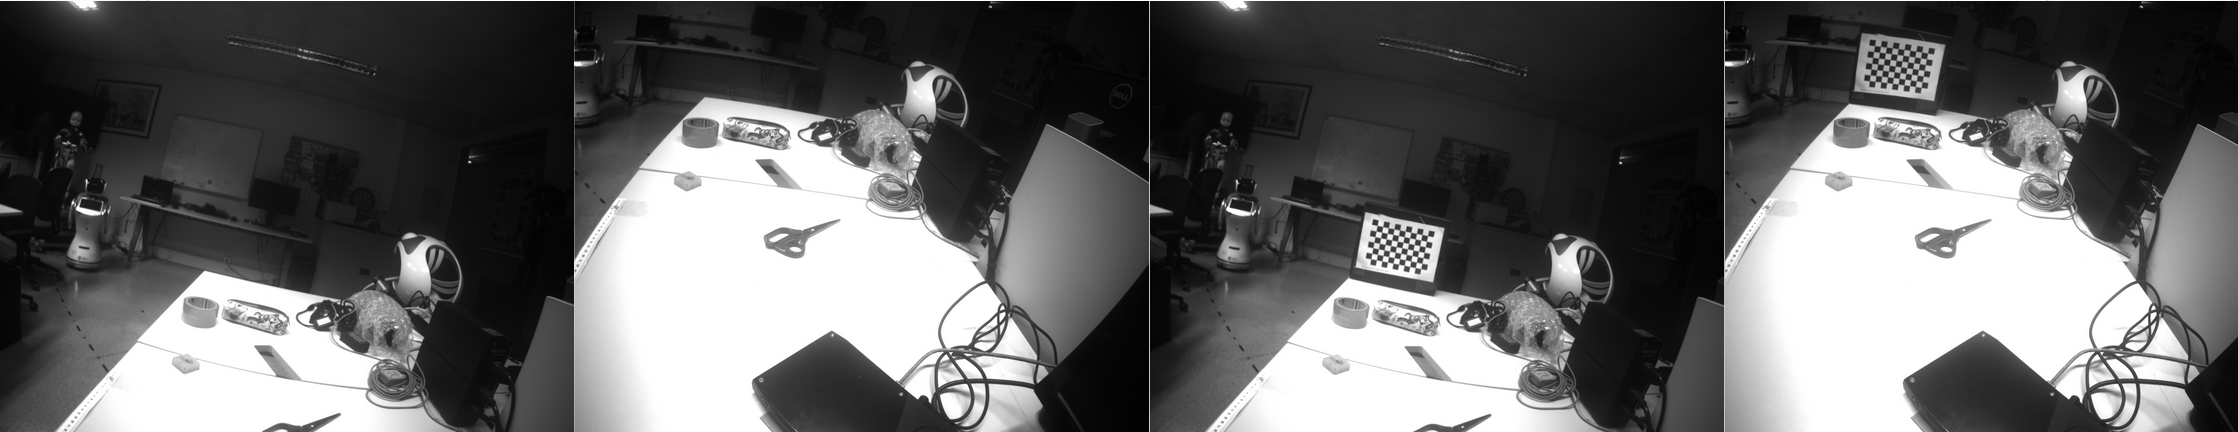
\includegraphics[width=\textwidth]{images/imagesex.png}
	 \caption[Example of the two pairs of images]{Example of the two pairs of images. The first and second images are used for finding feature matches and estimating the orientation. The third and fourth images are the same as the first and second ones, respectively, but with a chessboard positioned on the scenery, and serve as ground truth to evaluate the algorithms and the \acrshort{imu}'s performance.}
	 \label{cha3:methodology:imagesex}
 \end{figure}
	 
	 \item \textbf{Collect \acrshort{imu}}\\
	 The \acrlong{imu} \footnote{See appendix \ref{appendix:cha2:imu} for \acrshort{imu} specifications.} obtains two quaternions (see section \ref{cha2:represent:quat}) with the current camera's orientation before and after rotating.
	 
	\item \textbf{Find features and matches}\\
	As stated on section \ref{cha2:features} of the previous chapter,
	\acrshort{sift} and \acrshort{surf} seemed to be the most promising algorithms to detect features on the collected images. Because \acrshort{surf} is faster and more accessible due to patenting concerns regarding \acrshort{sift}, it will be be used on this work.
	\acrshort{flann} also previously referred to in the state of the art will be used for matching the features gathered between the two images, originating a set of point matches. The set of $N$ points matches are pixel coordinates in the first and the second image, $\mathbf{m_{1i}} = [u_{1i} \ v_{1i}]$ and $\mathbf{m_{2i}} = [u_{2i} \ v_{2i}]$, respectively, where $i=1,...,N$.
	
	\item \textbf{Filter outliers}\\
	
	
\end{enumerate}


\begin{figure}[ht]
	\centering
	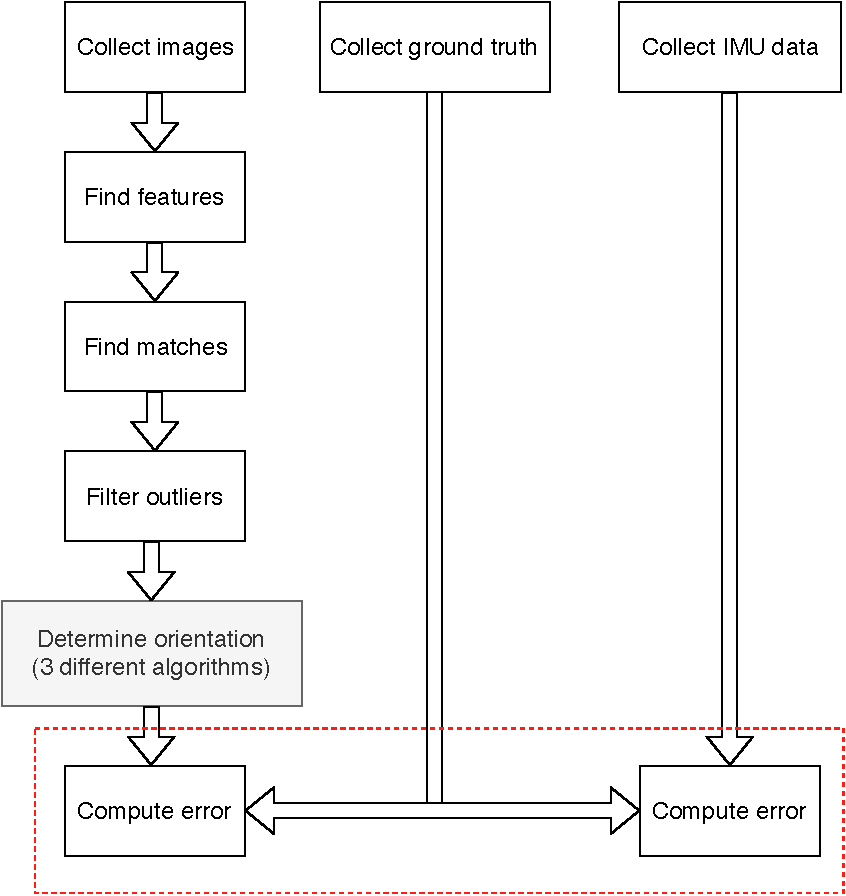
\includegraphics[width=0.7\textwidth]{images/approach.pdf}
	\caption[Approach Diagram]{Approach Diagram. Using the \acrshort{rgb} camera, two images are collected, before and after rotation. In each image, features are detected and matched between them. Some matches might be false or have too much noise, so they are filtered out. Using the matches information, the orientation is determined using an estimation algorithm. 3 algorithms will be put to test. Finally, the orientation determined is compared against the ground truth. The \acrshort{imu}'s orientation output is also compared against the ground truth to evaluate the improvement in relation to the camera.}
	\label{cha3:methodology:approach}
\end{figure}


\subsection{Feature detection and matching}

\subsection{Filtering matches}

\subsection{Determine orientation}

\subsubsection{Translation derivation}

As mentioned before, because the current eye prototype is a coupled system, the translation can be obtained through the knowledge of the rotation and the baseline length. This length is defined as the distance from the center of the camera's sensor to the center of rotation, as shown on Figure
\ref{cha3:detori:translation}.

\begin{figure}[ht]
	\centering
	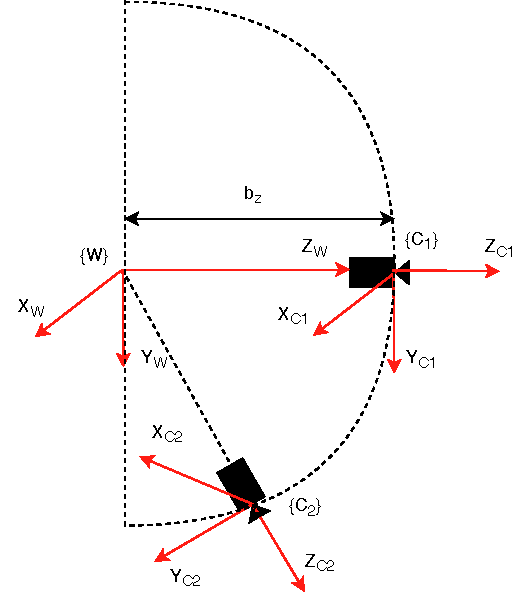
\includegraphics[width=0.5\textwidth]{images/transf.pdf}
	\caption[Translation derivation]{Translation derivation. Effect of a rotation on the current eye prototype's coupled system. The rotation and the baseline length define the translation. ${W}$ is the world reference frame centered on the rotation center, ${C_1}$ is the reference frame of the camera in the first position and ${C_2}$ is its frame on the second position, after rotating. $b_z$ is the baseline length on the Z axis.}
	\label{cha3:detori:translation}
\end{figure}

The translation can be easily derived as follows using frame to frame transformations\footnote{Consult Chapter 2 of Introduction to ROBOTICS mechanics and control \cite{robotics} on Spatial descriptions and transformations}. Having the world reference frame, ${W}$, set at the center of rotation, the transformation from the world to the first position of the camera, ${C_1}$, is

\begin{equation}
^W_{C_1}T = \begin{bmatrix}
I & -\mathbf{b}\\ 
\mathbf{0} & 1
\end{bmatrix},
\end{equation} 

where $I$ is the identity matrix and $\bf b$ is the baseline length expressed in each axis, $X$, $Y$ and $Z$, as $\mathbf{b} = [b_X \ b_Y \ b_Z]$. 

The transformation from the world reference frame to the second position of the camera, ${C_2}$, is
\begin{equation}
^W_{C_2}T = \begin{bmatrix}
R & -\mathbf{b}\\ 
\mathbf{0} & 1
\end{bmatrix},
\end{equation}\\
where $R$ is the rotation.

Hence, the transformation from the first position of the camera to the second can be obtained as
\begin{equation}
^{C_1}_{C_2}T = ^{W}_{C_2}T ^{C_1}_{W}T = ^{W}_{C_2}T ^{W}_{C_1}T^{-1} = 
\begin{bmatrix}
R & -\mathbf{b}\\ 
\mathbf{0} & 1
\end{bmatrix}
\begin{bmatrix}
I & \mathbf{b}\\ 
\mathbf{0} & 1
\end{bmatrix}
=
\begin{bmatrix}
R & R\mathbf{b}-\mathbf{b}\\ 
\mathbf{0} & 1
\end{bmatrix}.
\end{equation}
And finally, the translation ends up as
\begin{equation}
\mathbf{t}(R, \mathbf{b}) = R\mathbf{b}-\mathbf{b} = (R-I)\mathbf{b}.
\end{equation}


\subsubsection{\acrlong{grat}}

por isto no background
SAY THAT EPIPOLAR IS GOOD CUZ NO NEED TO DETERMINE Z, reference PAMI paper
IN TERMS OF R INSTEAD OF F
\subsubsection{\acrlong{mbpe}}
\label{MBaPE}
This method is a bundle adjustment of the previous one. It uses the rotation matrix obtained with OPPr and it tries to tune it to obtain a rotation and a translation dependent on the former, through 
\begin{align*}
	& \min_{R, Z_{e11}, ..., Z_{e1N}} \sum^N_{i=1} [(u_{e1i}-u_{1i})^2 + (u_{e2i}-u_{2i})^2 + (v_{e1i}-v_{1i})^2 + (v_{e2i}-v_{2i})^2]\\
	& \text{with} \ Z_{e1init} = \frac{1}{\sqrt{u_{1i}^2 + v_{1i}^2 + 1}} \ \text{and} \ R_{init} = R_{oppr},
\end{align*}
where $u_{1i}$ and $v_{1i}$ are the image points of the Camera View 1, $u_{2i}$ and $v_{2i}$ are the image points of the Camera View 2, $u_{e1i}$, $v_{e1i}$, $u_{e2i}$ and $v_{e2i}$ are the corresponding image points estimations and $Z_{e1i}$ is the depth of the Camera View 1.\\
The image point estimations are obtained the following way
\begin{align*}
	\mathbf{m_{e1}} = \frac{KR^T(Z_{e2}K^{-1}\mathbf{m_2}) - R^Tt)}{Z_{e1}}\\
	\mathbf{m_{e2}} = \frac{KR(Z_{e1}K^{-1}\mathbf{m_1}) + t)}{Z_{e2}}.
\end{align*} The depth is initialized by projecting the image points in a sphere.

METHOD OF MINIMIZATION LEVEN-MAGEFQ

\subsection{Simulator}

\subsection{Real world}

\subsubsection{Ground Truth}

Explain how this works on opencv and reference papers. or put on state of the art?

\subsection{C++ Library}